
% convert resulting pdf file to png to include in Jupyter Notebook
% Using ImageMagick:
% convert -density 200 Simplified_Monopoly_Board.pdf Simplified_Monopoly_Board.png

\documentclass[tikz]{standalone}

\usepackage{tikz}
\usetikzlibrary{calc}
\usetikzlibrary{shapes.geometric}
\usepackage{arev}

\begin{document}
  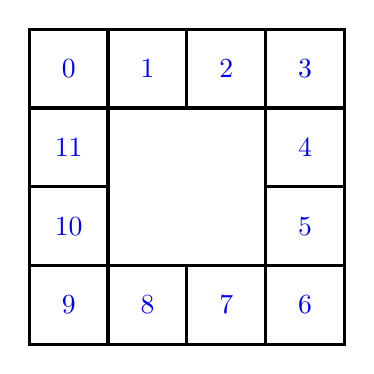
\begin{tikzpicture}[square/.style={regular polygon,regular polygon sides=4}]
    \newcommand{\squarenum}{0}
    \newcommand{\y}{3}
    \foreach \x in {0,1,2}
    {
      \draw[very thick] (\x,\y) +(-.5,-.5) rectangle +(.5,.5);
      \pgfmathtruncatemacro{\squareint}{\squarenum}  % turn into an integer
      \node[text=blue] at (\x,\y) {\squareint};
      \pgfmathparse{\squarenum +1}
      \xdef\squarenum{\pgfmathresult}
    }
    \newcommand{\x}{3}
    \foreach \y in {3,2,1}
    {
      \draw[very thick] (\x,\y) +(-.5,-.5) rectangle +(.5,.5);
      \pgfmathtruncatemacro{\squareint}{\squarenum}  % turn into an integer
      \node[text=blue] at (\x,\y) {\squareint};
      \pgfmathparse{\squarenum +1}
      \xdef\squarenum{\pgfmathresult}
    }
    \renewcommand{\y}{0}
    \foreach \x in {3,2,1}
    {
      \draw[very thick] (\x,\y) +(-.5,-.5) rectangle +(.5,.5);
      \pgfmathtruncatemacro{\squareint}{\squarenum}  % turn into an integer
      \node[text=blue] at (\x,\y) {\squareint};
      \pgfmathparse{\squarenum +1}
      \xdef\squarenum{\pgfmathresult}
    }
    \renewcommand{\x}{0}
    \foreach \y in {0,1,2}
    {
      \draw[very thick] (\x,\y) +(-.5,-.5) rectangle +(.5,.5);
      \pgfmathtruncatemacro{\squareint}{\squarenum}  % turn into an integer
      \node[text=blue] at (\x,\y) {\squareint};
      \pgfmathparse{\squarenum +1}
      \xdef\squarenum{\pgfmathresult}
    }
    
    
  \end{tikzpicture}

  
\end{document}
